\documentclass[9pt,a4paper]{beamer}
%\usepackage[utf8]{inputenc}
\usepackage[output-decimal-marker={,}]{siunitx}
\usepackage[compat=1.1.0]{tikz-feynman}
\usepackage{amsmath}
\usepackage[most]{tcolorbox}
\tikzfeynmanset{every blob = {minimum size = 2mm}}

\newcommand{\commento}[1]{}
\setbeamercolor{block title}{fg=white, bg=orange}

\beamertemplatenavigationsymbolsempty

%TITOLO TESI
%\usetheme{Madrid}
\usetheme{CambridgeUS}
\author[Adriano Del Vincio]{Adriano Del Vincio 562946\\ \footnotesize Relatori: prof. Francesco Forti, Prof. Concettina Sfienti}
\institute[Università di Pisa]{\textbf {Università di Pisa}}
\title[Tesi di Laurea]{Commissioning and First Data Analysis of the Mainz Radius Experiment}
\subtitle{}
\date{20/07/2023}
\titlegraphic{
\includegraphics[width=0.3\textwidth]{MarchioUnipi.pdf}}
\setbeamerfont{title}{shape=\itshape,family=\rmfamily}

\begin{document}
\setlength{\belowdisplayskip}{0pt}
\setlength{\abovedisplayskip}{0pt}


%TITOLO 
\frame{\titlepage}


% 1 INTRODUZIONE MREX 
\begin{frame}{The Mainz Radius Experiment}
\framesubtitle{MREX}

The Mainz Radius Experiment is an experimental campaign at the nuclear physics institute of Mainz, with the aim of investigating the properties of nuclear matter with imbalance in the number of protons and neutrons.

\begin{block}{Objective}
Determination of the neutron spacial density for $^{208}Pb$ nucleus, through the elastic electron scattering. From an accurate determination of the neutron spacial distribution, the \textit{Neutron Skin Thickness} of $^{208}Pb$ is measured.
\end{block}

\begin{columns}[T]
\begin{column}{.7\textwidth}
The results of the experiment will be valuable to constrain the Equation of 	State (EOS) of nuclear matter. It has also implications for the structure of neutron 		star.
\end{column}
\begin{column}{.3\textwidth}
\centering
\includegraphics[width = 0.75\textwidth]{figures/lead.pdf}
\end{column}
\end{columns}
\end{frame}

% 3 MREX e Neutron Skin
\begin{frame}{MREX and Neutron Skin Thickness}

\begin{definition}
The neutron skin thickness is defined as the difference between rms radius of neutron and proton spacial distributions:
\begin{equation}
\delta r_{np} = \sqrt{\vphantom{r^{2}_{p}}<r^{2}_{n}>} - \sqrt{<r^{2}_{p}>} ,
\end{equation}
\end{definition}

\begin{columns}[T]
\begin{column}{.5\textwidth}
In neutron rich nuclei, the spacial distribution of neutrons in more extended than proton spacial distribution.
Theoretical models link the Neutron skin thickness of heavy nuclei, such as $^{208}Pb$, with the \textbf{slope of the symmetry energy L}.
\end{column}
\begin{column}{.5\textwidth}
\centering
\includegraphics[width = 1\textwidth]{figures/SpacialDistribution.png}
\end{column}
\end{columns}
\end{frame}

% 4 SLOPE OF THE SYMMETRY ENERGY
\begin{frame}{Symmetry Energy}

The symmetry energy $S(\rho)$ is the key component of the equation of state which controls the neutron skin thickness. $S(\rho)$ quantifies the change in energy related to the neutron-proton asymmetry. 

\begin{equation}
\begin{split}
\epsilon(\rho, \alpha) &= \epsilon_{SNM}(\rho) + \alpha^{2} S(\rho) + O(\alpha^{4}) \\
\epsilon(\rho) &= J + L \cdot (\dfrac{\rho - \rho_{0}}{3 \rho_{0}}) + ...
\end{split}
\end{equation}

Cosa è l'energia di simmetria, come è collegata con il comportamento della materia nucleare di neutroni 

\begin{center}
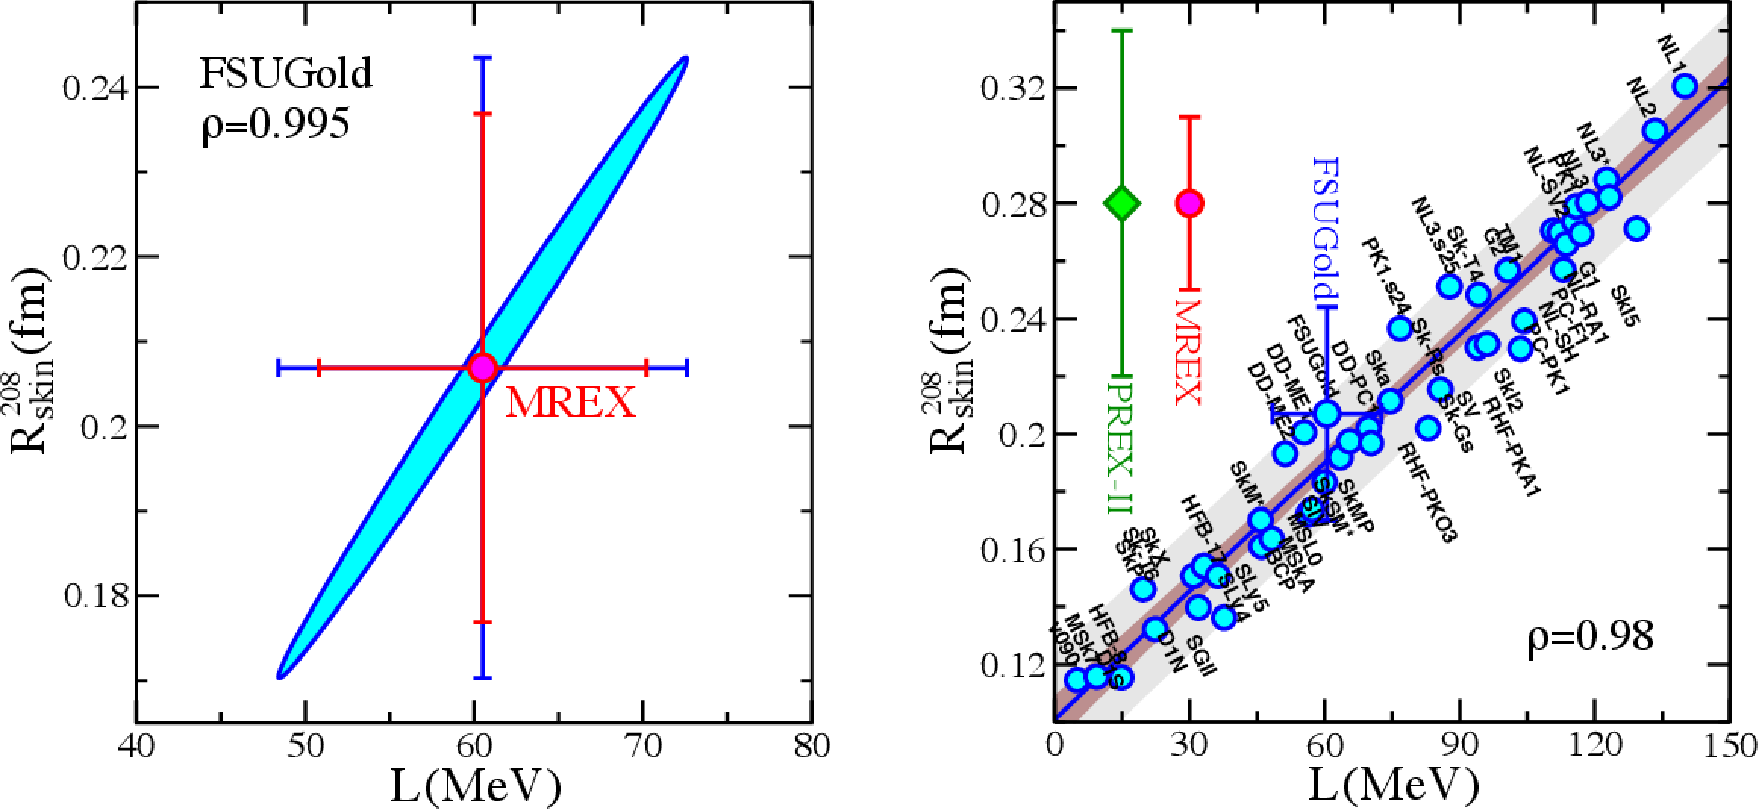
\includegraphics[scale=0.3]{figures/LvsR.pdf}
\end{center}

\end{frame}

% 5 Neutron Skin and Neutron Star Radius
\begin{frame}{Neutron Skin and Neutron Star Radius}
\begin{columns}[T]
\begin{column}{.5\textwidth}
The slope of the symmetry energy is related to both the neutron skin of lead and neutron star radius. The radius of the neutron star is determined from the Tolman–Oppenheimer–Volkoff (TOV) equation. Giving the pressure $P_{c}$ at the center of the star, the radius $R$ can be determined. But for neutron star, the pressure at the center is strongly related to the pressure of pure neutron matter, in large part determined by $L$.
\end{column}
\begin{column}{.5\textwidth}
\centering
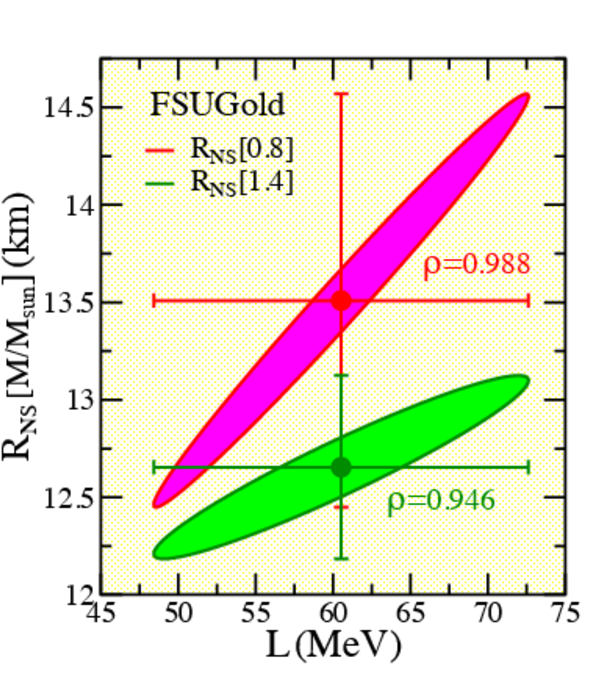
\includegraphics[scale=0.50]{figures/LvsRns.pdf}
\end{column}
\end{columns}
\end{frame}


% 6 Neutron Skin, misurare la densità spaziale di neutroni del nucleo di Piombo
\commento{
\begin{frame}{Measurement of the Neutron Spacial Distribution of Lead}

Misura della densità spaziale di neutroni, cenno ai limiti degli esperimenti con particelle alpha e pioni. Introduzione alla Parity Violating asymmetry.

\end{frame}}

% 7 PARITY VIOLATING ASYMMETRY
\begin{frame}
\frametitle{Parity Violating Asymmetry}
\framesubtitle{Measurement of the Neutron Spacial Distribution of Lead}

The determination of the neutron spacial distribution relies on the electron nucleus elastic scattering experiment, planned at the future MESA accelerator, in Mainz. 
The neutron spacial distribution is measured via the parity violating scattering, where longitudinal polarized electrons scatter from a fixed lead target. The key quantity is the asymmetry in the cross-section due to the different polarization state of the beam,

\begin{equation}
A_{pv} = \dfrac{\sigma_{R} - \sigma_{L}}{\sigma_{R} + \sigma_{L}}
\end{equation}

The asymmetry is due to the interference between two Feynmann diagrams.

\begin{figure}
\[
\feynmandiagram [scale =  0.8, transform shape][vertical = c to d]{
	a [particle = \(e^{-}\)] -- [fermion, thick] c -- [fermion, thick] g [particle = \(e^{-}\)],
	c -- [photon, edge label' = \(\gamma\), momentum = {[arrow style = blue]\(k\)}] d,
	h [particle = \(^{12}C\)] -- [fermion, thick] d -- [fermion, thick] j [particle = \(^{12}C\)],
	};
\qquad \qquad
\feynmandiagram [scale = 0.8, transform shape][vertical = c to d]{
	a [particle = \(e^{-}\)] -- [fermion, thick] c -- [fermion, thick] g [particle = \(e^{-}\)],
	c -- [photon, edge label' = \(Z\), momentum = {[arrow style = blue]\(k\)}] d,
	h [particle = \(^{12}C\)] -- [fermion, thick] d -- [fermion, thick] j [particle = \(^{12}C\)],
	};
\]
\end{figure}
\end{frame}

% 8 INTRODUZIONE ALLA TRANSVERSE ASYMMETRY
\begin{frame}{Transverse Asymmetry}

Argomento principale della tesi: misura dell'asimmetria trasversa, fondo sistematico di $A_{pv}$ da determinare. Introduzione alla fisica del processo 
\\ 
The transverse asymmetry is defined as the ratio between the sum and the difference of the elastic cross section for the two different polarized electrons: 

\begin{equation*}
A_{transverse} = \dfrac{\sigma_{\uparrow} -  \sigma_{\downarrow}}{\sigma_{\uparrow} + \sigma_{\downarrow}}
\end{equation*}

Before moving on to the experimental details, we identify the kinematics of the experiment. For the beam normal single spin asymmetry, the electrons are polarized in the normal plane identified by the $\frac{\vec{k'} \wedge \vec{k}}{ |\vec{k}| |\vec{k'}|}$

\begin{figure}[hbtp]
\[
\feynmandiagram [scale = 0.8, transform shape][vertical = c to d]{
	a [particle = \(e^{-}\)] -- [fermion, thick] c -- [fermion, thick] g [particle = \(e^{-}\)],
	c -- [photon, edge label' = \(\gamma\), momentum = {[arrow style = blue]\(k\)}] d [blob],
	h [particle = \(^{12}C\)] -- [fermion, thick] d -- [fermion, thick] j [particle = \(^{12}C\)],
	};
\qquad \qquad \qquad
\feynmandiagram [scale = 0.8, transform shape][baseline = (h), horizontal = d to j]{
	a [particle = \(e^{-}\)] -- [fermion, thick] c -- [fermion, thick, edge label' = \(e\), momentum = {[arrow style = blue]\(k_{1}\)}] f -- [fermion, thick] g [particle = \(e^{-}\)],
	c -- [photon, edge label = \(\gamma\)] d [blob],
	f -- [photon, edge label = \(\gamma\)] j [blob],
	h [particle = \(^{12}C\)]-- d -- [fermion, thick] j -- k [particle = \(^{12}C\)] ,
	};
\]
\end{figure}
\end{frame}

% 9 DESCRIZIONE DEL PROCESSO
\begin{frame}{Description of the Process}

The transverse asymmetry arises considering the time reversal operator. The time reversal operator reverses all the momenta and the spin direction.

\begin{figure}[hbtp]
\centering
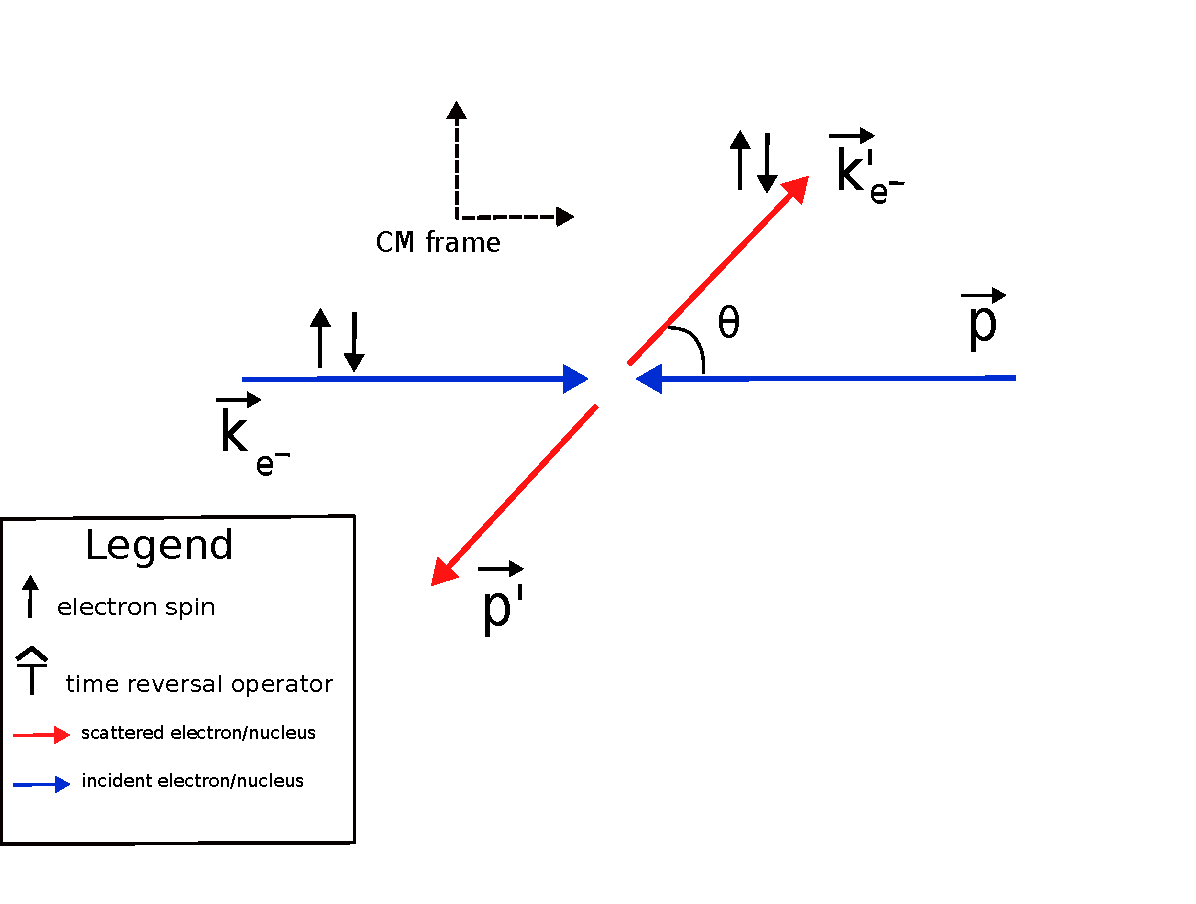
\includegraphics[width = 0.8\textwidth]{figures/ScatteringScheme.pdf}
\end{figure}


\end{frame}

\begin{frame}{Scattering Process}

The incident beam is made by $\SI{570}{\mega \electronvolt}$ electrons, that are polarized along the transverse axes ($\uparrow$ and $\downarrow$). The physical quantity to measure is the asymmetry between the number of scattered electrons, due to the change of the polarity:

\begin{equation}
asym = \frac{N_{+} - N_{-}}{N_{+} + N_{-}} \text{(expected $\sim$ +/- 20 ppm, Q = \SI{0.2}{\giga\electronvolt c^{-1}})}
\end{equation}

It's possible to obtain a final formula for the transverse Asymmetry, writing the Amplitude of the 1-loop diagram, considering the elastic intermediate state and the inelastic intermediate state (whose contribution is higher):

\begin{equation}
A_{n} \simeq C_{0} \log \frac{Q^{2}}{m^2_e c^2} \frac{F_{Compton} (Q^2)}{F_{ch}(Q^2)}
\end{equation}

MENZIONARE PREX!!!

\end{frame}


% 10 BEAM TIME, OBIETTIVI DELL'ESPERIMENTO
\begin{frame}{Beam-time 29/11/2022 - 5/12/2022}
\framesubtitle{Beam Normal Single Spin Asymmetry at MAMI}
During the last beam-time, several measurements were performed at Mainz Mikrotron MAMI. The last data acquisition campaign had the following goals:

\begin{itemize}
\item Test the new data acquisition system, developed for the new setup with a low rate signals ($\simeq \SI{1}{\mega \hertz} $). 
\item Measure the transverse asymmetry $A_{n}$ of $^{12}C$.
\item Measure the expected rates on $^{208}Pb$ target, in anticipation of the future measurement of $A_{n}$ for lead. 
\item Long term goal: acquire more knowledge on the systematic effects that the transverse asymmetry has on the measurement of the Parity-violating asymmetry.
\end{itemize}
\end{frame}

% 15 Struttura dell'evento
\begin{frame}{Structure of the event}

The Data are divided in a series of events (\SI{80}{\milli \second}), that correspond to 4 sequential sub-event. For each sub-event there is a precise polarization of the Beam. For each sub-event all the scattering electrons are counted.uring . 

\begin{figure}[hbtp]
\centering
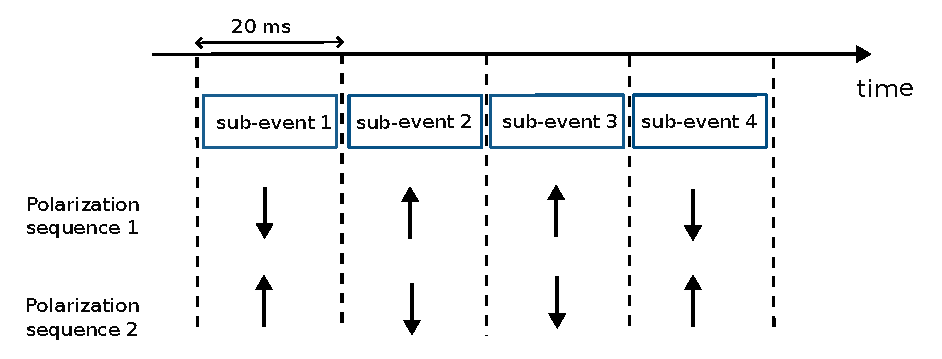
\includegraphics[width = 0.75\textwidth]{figures/EventStructure.pdf}
\caption{Event sequence: all the particle}
\end{figure}

\end{frame}

% 11 MAMI ACCELERATORE
\begin{frame}{MAMI Electron Accelerator}

Schema dell'acceleratore e descrizione breve del suo funzionamento

\end{frame}

% 12 Sala Sperimentale
\begin{frame}{Experimental Hall}

Immagine A1.

\end{frame}

% 13 SCHEMA DETECTORS

\begin{frame}{Detectors}

\begin{figure}[!hbtp]
\centering
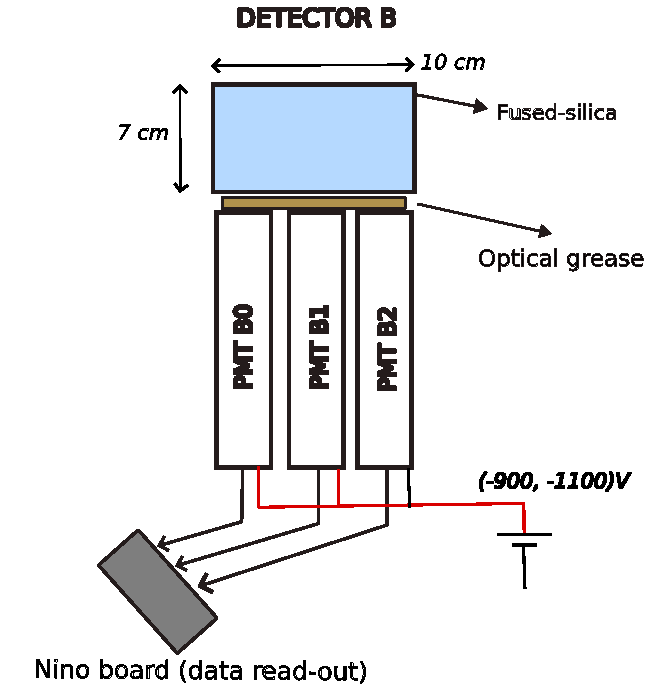
\includegraphics[width = 0.4\textwidth ]{figures/DetectorB.pdf}
\hspace{1cm}
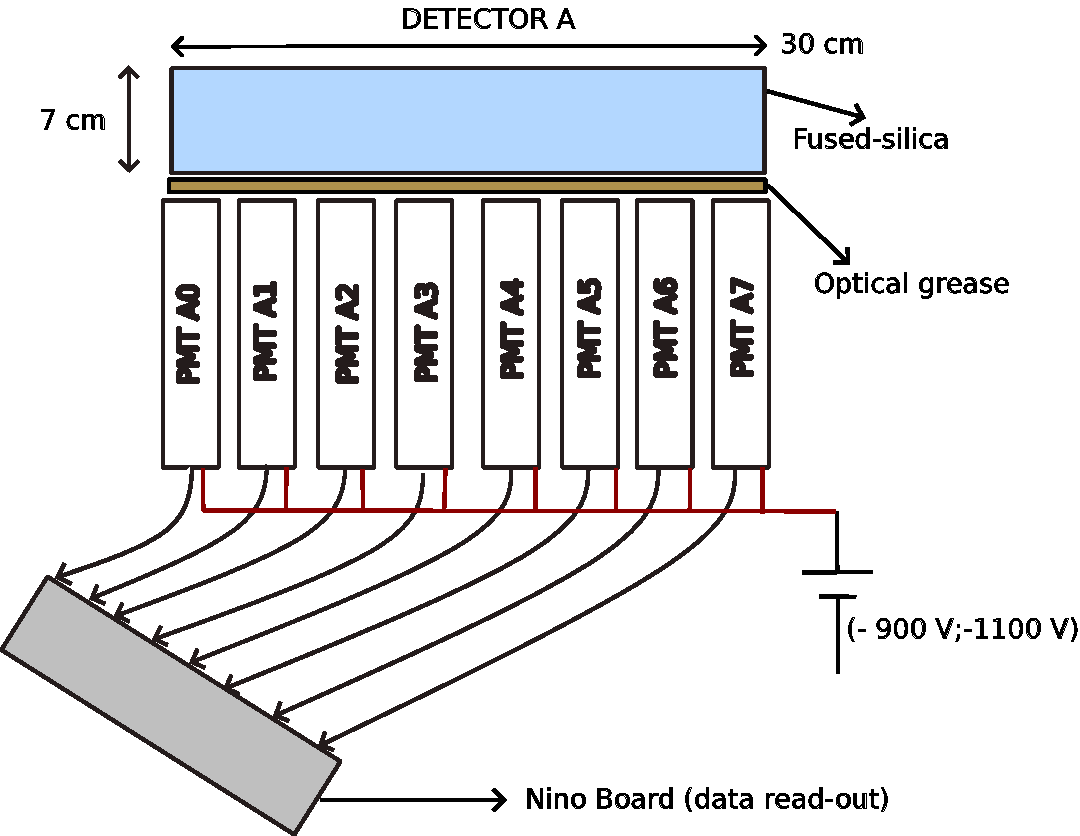
\includegraphics[width = 0.5\textwidth ]{figures/detectorA.pdf}
\end{figure}

\commento{The detectors are made by 9 and 3 pmts coupled to a fused-silica material, exploiting the Cherenkov light produced when a particle travel inside the material.

\begin{figure}[hbtp]
\centering
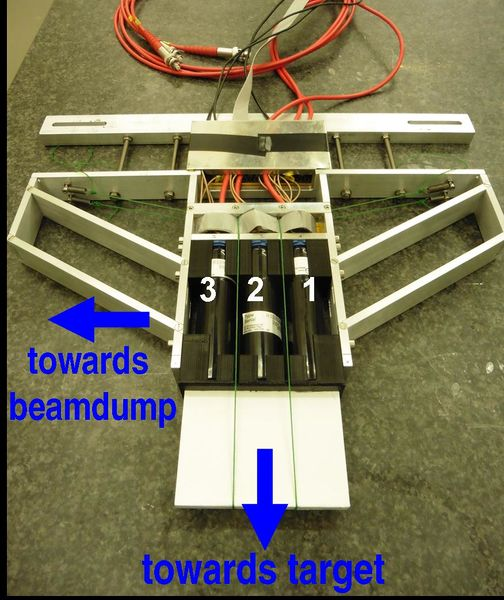
\includegraphics[width = 0.3\textwidth]{figures/504px-Blackfalcon.jpg}
\hspace{2cm}
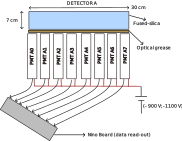
\includegraphics[width = 0.4\textwidth]{figures/DetectorA.jpg}
\caption{Detector B on the left, detector A on the right.}
\end{figure}}

\end{frame}

% 14 NINO BOARD
\begin{frame}{NINO Board}

Nino board, immagine + spiegazione di come sono acquisiti i segnali.

\end{frame}

% 16 Problema delle false asimmetrie
\begin{frame}{False Asymmetries}
The counts of the pmts can be slightly different due to the variation of the position of the beam on the target, the variations of the incident angles, the uncertain associated with the energy and the current of the beam. All this quantity can influence the asymmetry measured by the pmts, considering also that the expected asymmetry is in the order of ten part per million, and small asymmetry introduced by fluctuations of the beam parameters are not negligible:
\newline
\newline
\begin{equation}
Asym = A_{physical} \cdot P + \delta_{I} + A_{x} \delta x + A_{y} \delta y + A_{\theta_{x}} \delta \theta_{x} + A_{\theta_{y}} \delta \theta_{y}+ A_{E} \delta E 
\end{equation}
\end{frame}


\begin{frame}{MAMI Beam Monitors}

Descrizione dei principi di funzionamento dei monitors di MAMI.

\end{frame}


\begin{frame}{Voltage to Frequency Converter}

Breve descrizione di come funzionano i voltage to frequency converter

\end{frame}

% 17 SCHEMA GENERALE DELL'ESPERIMENTO
\begin{frame}{General Scheme of the Experiment}

\begin{figure}[hbtp]
\centering
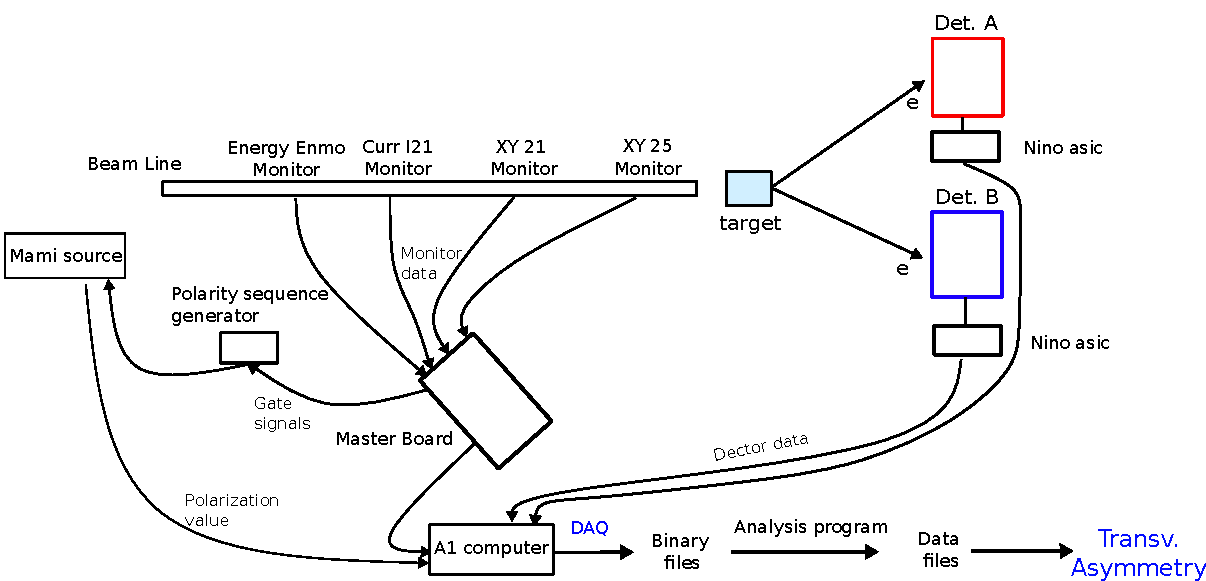
\includegraphics[width = 0.9\textwidth]{figures/Electronic_scheme.pdf}
\caption{Scheme of the experiment.}
\end{figure}
\end{frame}

% 18 1 DETECTOR TEST
\begin{frame}{Detector Tests}

\end{frame}

% 18 CALIBRATION OF THE BEAM PARAMETERS
\begin{frame}{Calibration of the Beam Parameters}

\end{frame}

\begin{frame}{Beam Position}

\end{frame}

\begin{frame}{Beam Energy}

\end{frame}

\begin{frame}{Beam Current}

\end{frame}

\begin{frame}{Auto-Calibration procedure}

\end{frame}

% 19 DATA ANALYSIS
\begin{frame}{Analysis on Carbon Target}

\end{frame}

% 20 Model for Fitting the Data
\begin{frame}{Model For Fitting the Data}

Modello lineare tra asimmetria e beam parameters, discutere differenza corrente e altri parametri del fascio. 

\end{frame}

% 21 Data Selection
\begin{frame}{Data Selection}



\end{frame}

% 22 Polarization Loss
\begin{frame}{Polarization Loss}

Discutere la rilevante perdita di polarizzazione che è avvenuta ed il modo in cui si sono identificati questi dati.

\end{frame}

% 23 FIT TO DATA, CORRELATION
\begin{frame}{Beam Parameters Correlation}

\end{frame}

% 24 EXPECTED ERROR
\begin{frame}{Variance of the Asymmetry Data}

The statistical error of the measured asymmetries is now computed:

\begin{gather*}
Var[A_{asym}] = Var[\dfrac{N_{\uparrow} - N_{\downarrow}}{ N_{\uparrow} + N_{\downarrow}}] \simeq \dfrac{Var[N_{\uparrow} - N_{\downarrow}]}{(N_{\uparrow} + N_{\downarrow})^{2}} \\
\frac{2Var[N]}{4N^{2}} = \frac{1}{2N} \qquad \sigma = \frac{1}{\sqrt{2N}}
\end{gather*}

Where it is supposed that the PMTs counts are normal distributed, with $\mu$ equal to $\sigma^{2}$. The rms associated to the sample mean decreases as the $\sqrt{N_{measure}}$. 

Considering $5\cdot 10^{5}$ events and $\mu = 40000$ counts per PMT (similar to what was measured for detector A) we obtain an error of $\simeq 5ppm$.

\end{frame}


\begin{frame}

Here a plot about the trend of the asymmetry as the data increases. The band is the error computed as showed in the previous slide, centered around the values of $+20ppm$ for detector A and $-20ppm$ for detector B.

\begin{figure}[hbtp]
\centering
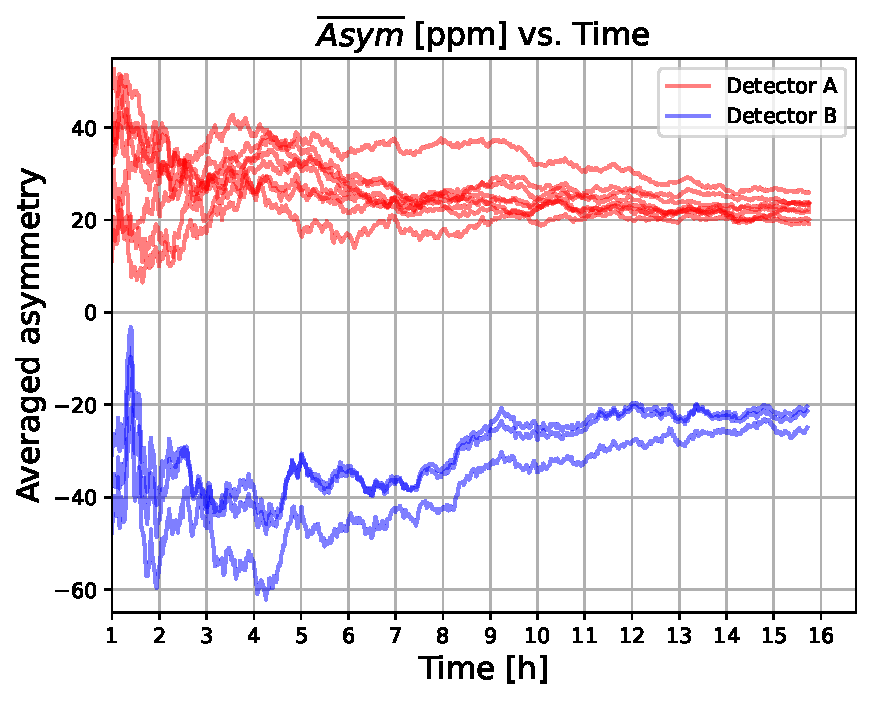
\includegraphics[width = 0.70\textwidth]{figures/AveragedAsymmetry.pdf}
\end{figure}

\end{frame}


% VISUALIZATION OF THE DATA
\begin{frame}{Visualization of the Data}

\end{frame}

\begin{frame}{Results}

For each pmt, we present the raw values of the asymmetry, obtained by subtracting the Raw current asymmetry, that is roughly $-1.11$ ppm , then we compute the averaged values:

\begin{figure}[hbtp]
\centering
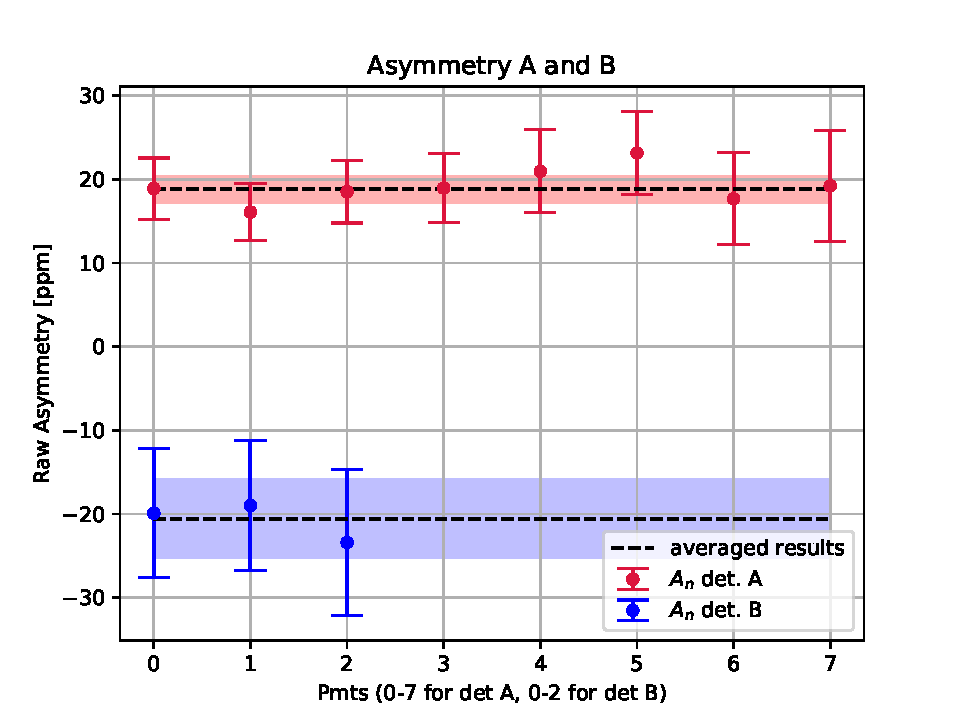
\includegraphics[width = 0.65\textwidth]{figures/FirstResult.pdf}
\end{figure}
\end{frame}

\begin{frame}{Results}
 
Combining the result of each pmt, assuming all the asymmetries measured are independent of each other, we obtain the following quantities for Beam normal single spin asymmetries:

\begin{gather*}
\hat{A} =  \frac{\Sigma_{i} A_{i} \frac{1}{w_{i}}}{\frac{1}{w_{i}}} \qquad w_{i} = \frac{1}{\sigma^{2}_{i}}
\end{gather*}

We obtain the following:
\begin{equation}
A_{A} = (23.1 \pm 1.7) ppm  \qquad A_{B} = (-21  \pm 5)ppm
\end{equation}

Reversing the sign of the asymmetry for detB we notice that the two measurement are consistent, and this show the good behaviour of the electronic setup used for the experiment. 

\end{frame}

\begin{frame}{Rates on Lead}
\begin{figure}[hbtp]
\centering
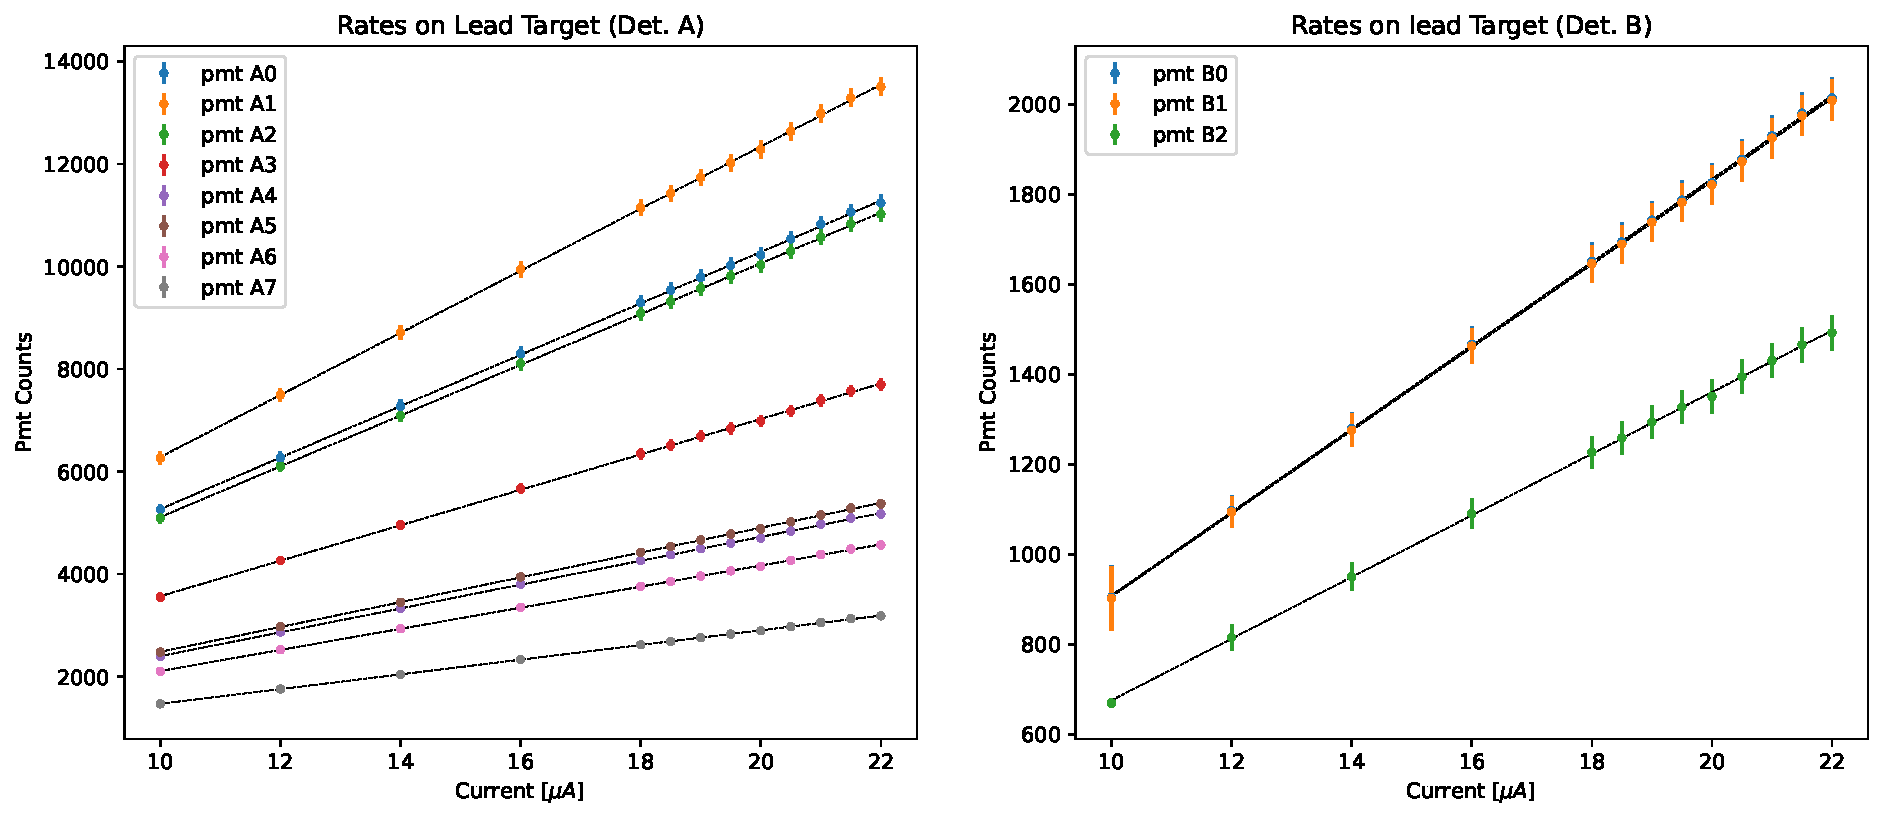
\includegraphics[width = \textwidth]{figures/LeadRates.pdf}
\end{figure}

\end{frame}

\end{document}